\chapter{Conclusions and Future Work}
\label{c:conclusions}

After the demonstration of \Fountain{} in previous chapter, we know that the proposal of \RRS{} system is feasible and has a great extensibility. We summarize the advantages of \RRS{} as follows:
\begin{enumerate}
\item \textbf{Leveraging the hardwares on the remote engine} ─ Because \RS{} could do the computation and graphics operation, it's better to run on the more powerful hardwares. Unlike the other screen sharing mechanism, we fully exploit the power of the remote engine and relieve the network traffic. Only the RS command is necessary to send.
\item \textbf{No migration overhead} ─ The existing RS applications have almost no code necessary to be added or modified for migrating to \RRS{}. For instance, we migrate \Fountain{} without any overhead. Again, we are target for RS debugging framework, so the feature is important for \RRS{}.
\item \textbf{Debug for \RS{}} ─ \RRS{} speeds up the debugging progress no matter of using emulator or device. By punching through via \RRS{} and set up the environment, RS developer could have a better user experience on \RRS{} rather than the emulator. 
\end{enumerate}

%經過嚴密的測試之後,我們可以發現 RRS 這個框架的實作是一定可行的。而且有非常大的可擴充性,他有以下幾個好處:
%
%1. 充分的利用機器效能,效能表現不在受牽制於性能比較不可的程式
%因為 RS 同時可以繪圖與計算,不但需要強大的CPU 更需要強大的GPU,而往常的螢幕同步機制通常是把整個顯示在螢幕上的資訊壓縮然後整個傳輸過去,即使壓縮過後的 frame rate 可以提高,以會影響整個影像的品質,而我們不但可以充分的利用遠端引擎上的圖形硬體,還可以利用強大的計算能力,而不同的應用程式也會依其執行環境而擁有最佳表現。
%除此之外我們也讓網路的負擔最低,一旦把命令傳輸過去之後,就不再傳輸任何東西。
%
%2. 所有的應用程式不需要任何更動即可直接使用 RRS
%在 fountain 之中,我們沒有更動任何應用程式的程式碼,因為我們目標就是提供一個 framework,並且可以非常輕易的移植到 RRS 之上,這也是作為 debugger 所必要的一個特色。
%
%3. 解決 RS 沒有除錯機制的問題
%即使未來有了 emulator 支援了 open gl es 2.0 而可以跑 renderscript,因為整個是使用模擬出來的 arm (armv5),效能表現是相當差的,我們透過 RRS 間接的打穿,並且直接利用本機的圖形硬體加強了整體的效能表現。再透過 adb 設置好環境,就可以順利的江畫面傳送過去並進行除錯動作。
%
%4. 結合雲端應用的潛力
%除了除錯的應用以外,我們也在前面舉了相當多的例子,RS 未來最主要的應用或許是再遊戲,而現在手機非常普遍,未來多人連線「在地」遊戲或許會非常火紅,舉個例子來說,如果我們是完麻將遊戲,那麼麻將桌就是電視,電視連接四台手機,而每個手機則是自己的牌。透過 RRS 達成同步的機制,並且充分的各個手機的硬體效能,讓我們可以完美的實現三螢一雲,就如下圖,畫出我們整體的大方向。

\begin{center-figure}
	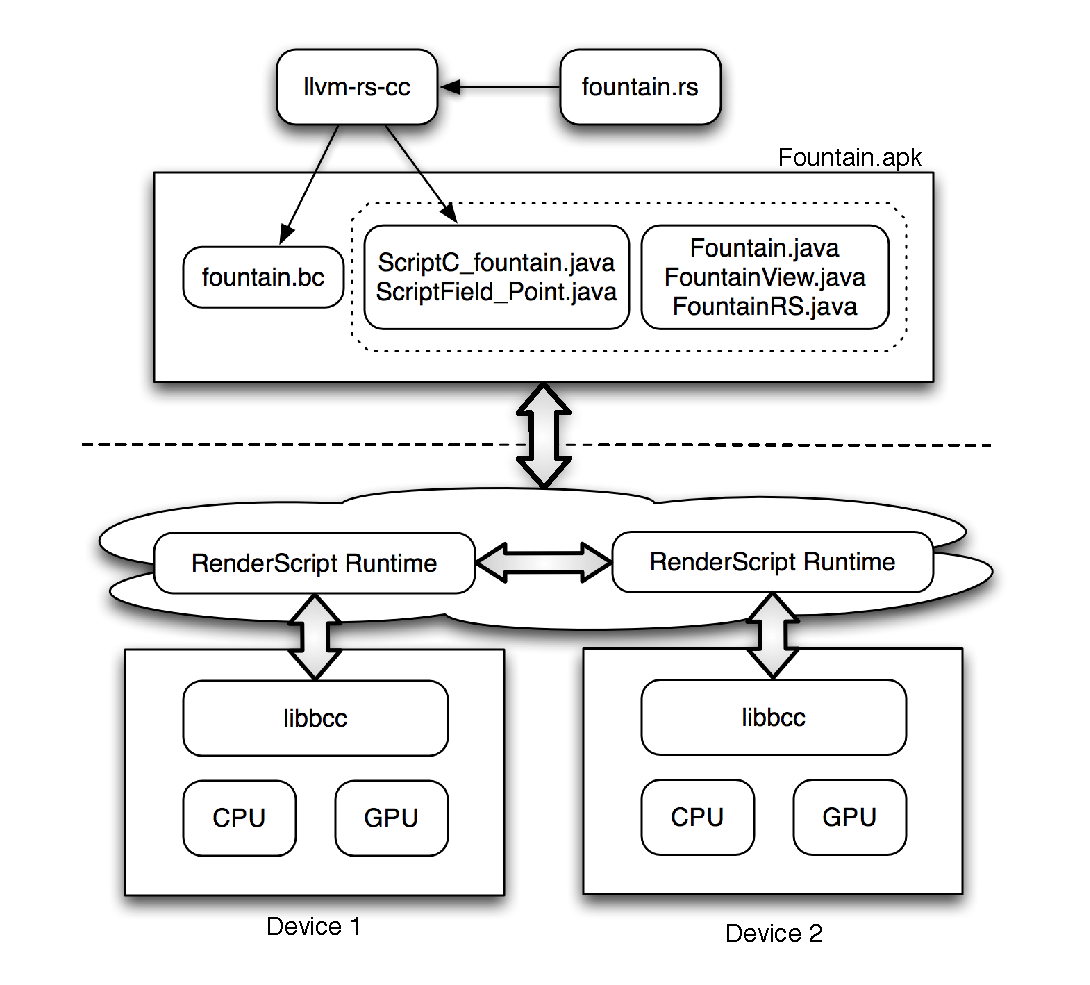
\includegraphics[scale=0.8]{fig/Future_RRS.eps}
	\caption{The big picture of Remote RenderScript}
	\label{fig:Future_RRS}
\end{center-figure}

It is just a \RRS{} prototype, there are still many stuff that we need work harder to perfect it in the future:

\begin{itemize}
\item \textbf{Heterogeneity among Devices} ─{} In the thesis, we just test \Fountain{} on the same devices. What if we communicate between two different devices? The size of screen might differ largely, e.g., smartphone and TV. Also, it must need a synchonization of screen size. We compute in individual devices, so we could scale the graphs up losslessly. The other easier approach is simply enlarging the window, but the resolution might be not satisfying. 
\item \textbf{Bi-directional Communication} ─{} One-way synchronization is not enough for non-debugging purposes. Our implementation is one-way by now, that is, one for sending and the other one for receiving only. In the future, we expect to extend it to have the ability of a two-way and one-to-many communication among devices. (As shown in Figure \ref{fig:StarCommunication} (a), and (b) respectively.) In other words, each device could be not only a client but also a server to facilitate our desirable personal-cloud.
\item \textbf{Application for Cloud Computing} ─{} As we said in Chapter \ref{c:intro}, gaming might are the main purpose of \RS{}. Of course, \RRS{} is suitable for game development. For instance, everyone might have one smartphone in the recent future. Game vendor could use \RRS{} to develop a multi-player game instread of tranditional board games, and replace the board with a larger screen device like TV. Our vision is similar with Google Project Tungsten.
\item \textbf{Security} ─{} Network pairing must be done to set up the environment for \RRS{}. For security concern, auto-pairing is not permitted. So the authentication is necessary in the future network-pairing process to eliminate security concern.
\end{itemize}


\begin{center-figure}
	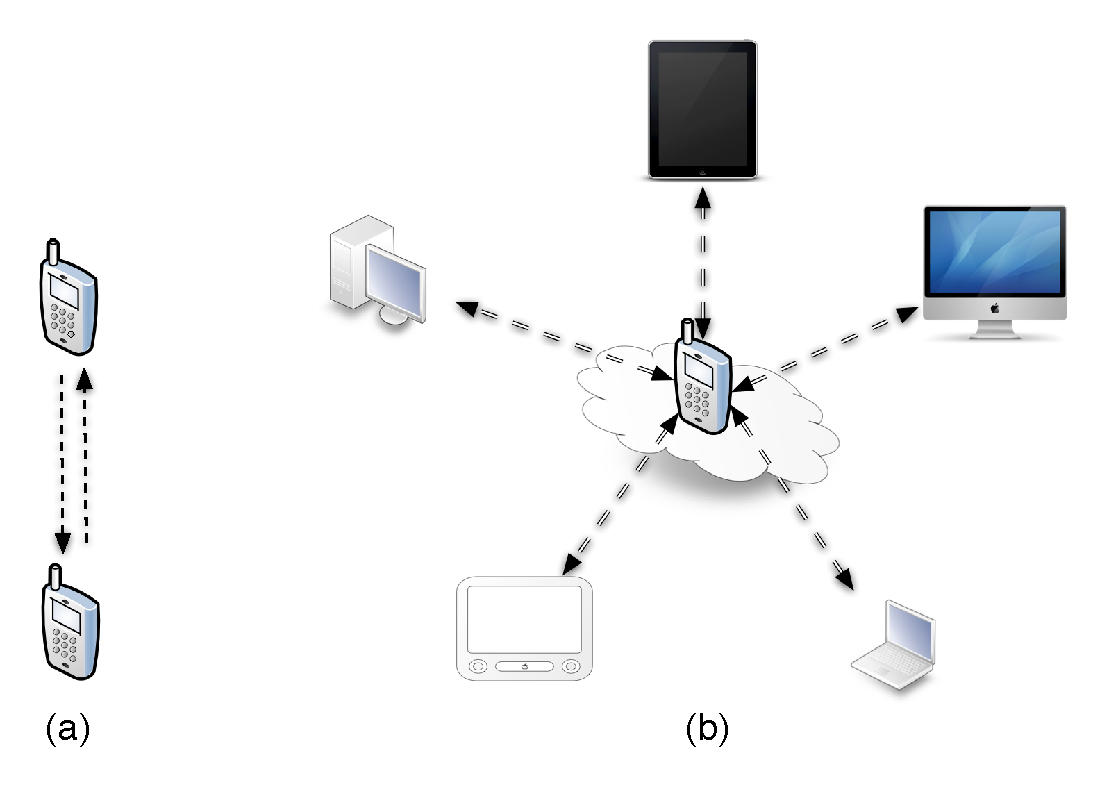
\includegraphics[scale=0.8]{fig/NetworkCommunication_Star.eps}
	\caption{Communication among hetrogeneous devices: (a) Bi-Direction (b) One-to-Many}
	\label{fig:StarCommunication}
\end{center-figure}
%1. Should we scle up when the remote has larger screen?
%目前我們測試是在兩隻相同的手機之上,但是如果未來是再不同裝置之間傳送,螢幕大小的差距可能會非常的大,例如手機與電視,那我們勢必要加上螢幕的同步處理,因為我們只是個指令,所以或許可以直接透過指令去分析,並且做不失真的圖形放大處理。另外一種比較簡單的作法就是單純的裝置上實作最大化視窗的功能,但是可能解析度的表現就不如上述方法還好。
%
%2. two-way synchronization
%如果要將 RRS 使用再非除錯的用途之上,單方向的傳送勢必是不足的,而目前我們的實作之中,只純粹的處理單方向同步,也就是 client-server 單一架構,未來的話,預計將其擴展,每個裝置本身同時可以是 server 也可以是 client,實現所謂的 personal-cloud 理想。
%
%3. Authentacation
%每個裝置連線時,我們必須事先做好網路pairing 的工作,但是我們不可以允許自動的配對,這會有安全性上的問題,所以未來如果我們要使用RRS 再一般應用之上(例如遙控播放),那麼我們就必須在其之上加入認證機制,解決安全性上的問題。

%--
%2. need to sync, should implement a network flush()
%cmd+1 is only if (dataLen < DATA\_SYNC\_SIZE), we should take care of other cases
%從前面我們可以了解到指令分為需要同步與不需要同步兩種,而在 Fountain 中,其需要的指令都是不必同步的,所以我們日後勢必還得處理同步問題。
%
%4. Now we only handle ScriptInvokeV(...). In other functions, there are must some pointer in the parameters (inconsistent memory addr).
%雖然整體來說需要傳送的指令種類不多,但是因為每個指令的參數都不一樣,而這種不同的參數都必須處理其記憶體位址問題,所以如果未來要將RRS 擴展,勢必也要將其他函式的問題解決
%
%5. Because ScriptCCreate is luckily the last "Create" command, we could get the pointer from mToCoreRet directly.
%--




